% =====================================================================================
% DA4022 final report -- NeurIPS 2026 template (Overleaf: "Formatting Instructions For
% NeurIPS 2026"). Plain-language version (jargon and verbosity removed, as the course allows).
% Every number is taken from results/ (tables via make_tables.py, figures via make_figures.py).
%
% STRICT 5-PAGE VERSION: main text + acknowledgements + references fit in 5 pages; there is no
% appendix. The longer version with an appendix is main_with_appendix.tex.
% =====================================================================================
\documentclass{article}

% [preprint] = non-anonymous version with the author names and the footer
% "Preprint. Work in progress." The default option (main track) is the anonymous
% double-blind submission and would hide the author names; [final] is reserved for
% papers accepted to NeurIPS. Keep the template's neurips_2026.sty unchanged.
\usepackage[preprint]{neurips_2026}

\usepackage[utf8]{inputenc} % allow utf-8 input
\usepackage[T1]{fontenc}    % use 8-bit T1 fonts
\usepackage{amsmath}        % \text, aligned math
\usepackage{graphicx}       % figures
\usepackage{adjustbox}      % tables shrink only if wider than the text
\usepackage{hyperref}       % hyperlinks
\usepackage{url}            % simple URL typesetting
\usepackage{booktabs}       % professional-quality tables
\usepackage{amsfonts}       % blackboard math symbols
\usepackage{nicefrac}       % compact symbols for 1/2, etc.
\usepackage{microtype}      % microtypography
\usepackage{xcolor}         % colors

\title{Quantifying Look-Ahead Bias via Causal, Volatility-Aware Motif Tokenization in Financial Time Series}

% AUTHOR ORDER: change it here only. (The 15 Oct midterm slide listed: Sanidhya Srivastava,
% Arnav Tiku, Devansh Jangid, Karan Malik, Aman Gupta.)
\author{%
  Devansh Jangid \quad Aman Gupta \quad Arnav Tiku \quad Sanidhya Srivastava \quad Karan Malik \\
  DA4022 Course Project \\
  \texttt{github.com/devanshjangid2005/causal-vol-tokenizer}
}

\begin{document}

\maketitle

% ------------------------------------------------------------------ Abstract
\begin{abstract}
Motif tokenizers turn a price series into tokens, much as BPE does for text. They are usually tested
on data they have never seen. When one is used to forecast a single market step by step through time,
it can quietly use information from the future: its settings may be fitted on test-period data, or a
token may reach past the moment of the forecast. We built a backward-looking pipeline for 5-minute
Bitcoin volatility and switched on one possible leak at a time against a matched control. Over six test periods (26,290
hourly forecasts, three training runs), letting the normalization window see the forecast period
lowers the forecast error (QLIKE) by 63.39\%, or 62.03\% when the periods are pooled, with the same
effect in every period. It is the only leak that beats the best possible score on simulated data. The
other four leaks change the error by at most 2.84\% one hour ahead, but grow one day ahead, where one
leak can hide the cost of another. A 2025 test set, run only once, confirms the normalization leak
($+73.90\%$).
\end{abstract}

% ------------------------------------------------------------------ 1. Introduction
\section{Introduction}

Motif tokenizers \citep{gotz2026bpe} round each value of a time series into one of a fixed set of bins
and then merge frequent pairs of bins into longer tokens. They are usually tested on new datasets. Forecasting one
market through time is different: every part of the pipeline is fitted on the same series that is
later forecast, so every part is a possible route for future information. Earlier work has shown
leakage between datasets and between related series \citep{meyer2025leakage}, but no one has measured
it part by part inside the tokenizer.

A leak can enter in two ways. At fitting time, the normalization, the merge table or the decoding
tables can be estimated on data that overlap the test period. At encoding time, the problem is that
BPE is not incremental: encoding the start of a series does not always give the start of the full
encoding \citep{zhang2026unitok}. If we tokenize the past and the future together and then cut at the
forecast time, the token that crosses the cut carries future data. If we tokenize only the past, the
last token may be cut short, which biases the next prediction; this is called partial-token bias
\citep{phan2024tokenization}.

We measure how much each leak inflates measured accuracy. We contribute a separate test of five leaks
against matched controls, a measurement of how two of them trade off, a tokenizer that never looks
ahead at forecast times on the hour, and a test design with controls, six test periods and a one-time
2025 test.

% ------------------------------------------------------------------ 2. Method
\section{Method}

\begin{figure}[t]
  \centering
  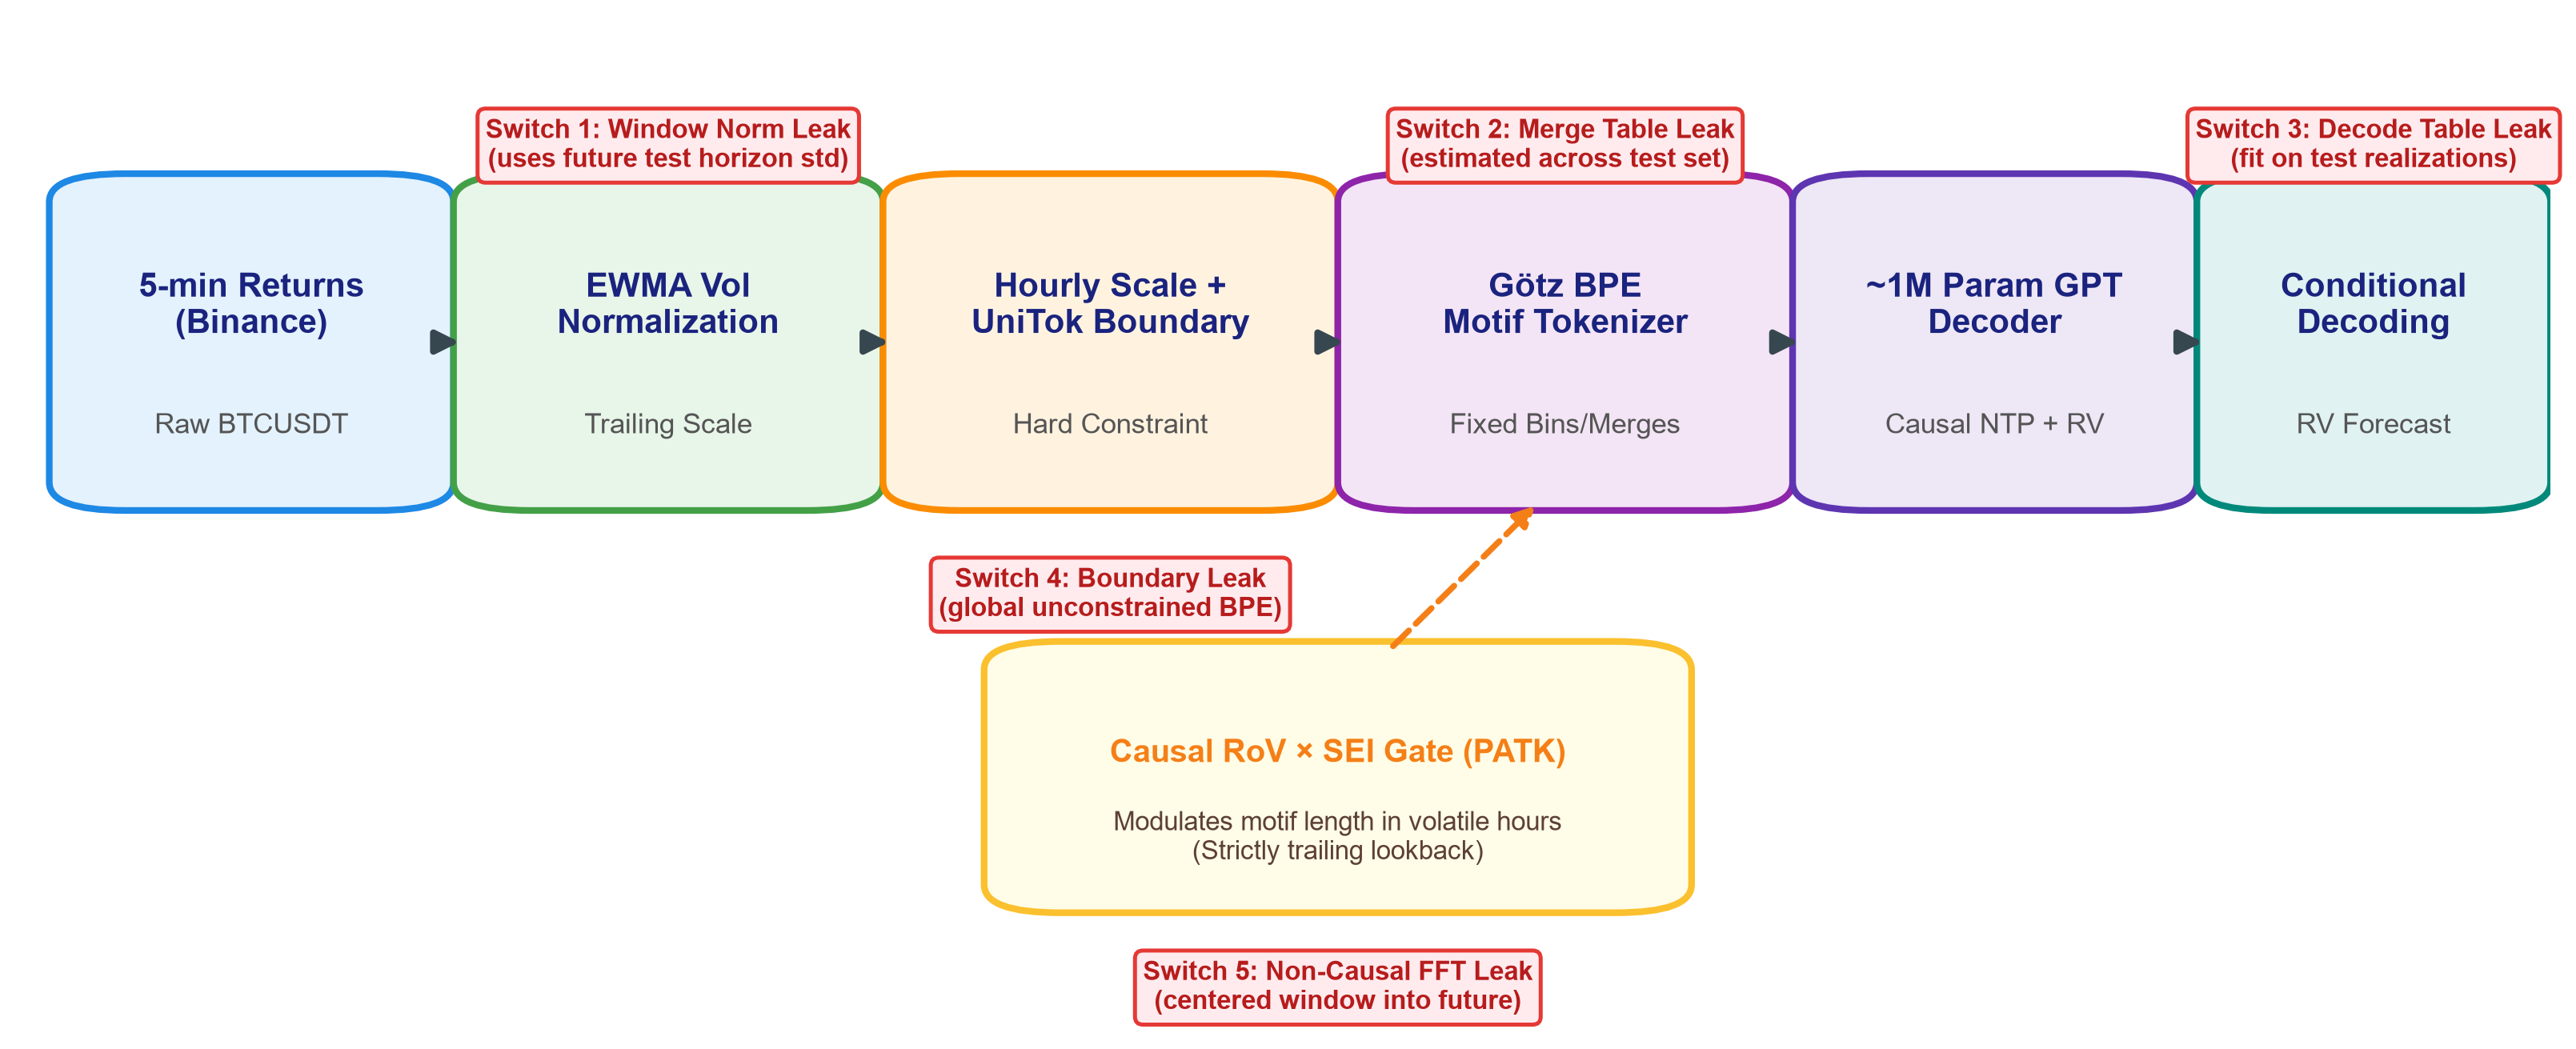
\includegraphics[width=0.92\linewidth]{figures/pipeline_leak_switches.png}
  \caption{Our leak-free pipeline and the five leak switches (red boxes). Each leak changes one
  setting, in both training and testing. The model has 855,169 parameters (the figure rounds this
  to 1M).}
  \label{fig:pipeline}
\end{figure}

\paragraph{Data and target.}
We use 5-minute Bitcoin (BTCUSDT) prices from Binance, January 2021 to December 2025. We compute log
returns, set returns across exchange outages to zero, and divide each return by a volatility estimate
that uses past returns only: $\sigma_t^2 = 0.94\,\sigma_{t-1}^2 + 0.06\,r_{t-1}^2$. A forecast made at
time $t$ may use data up to $t-1$. It predicts the realized variance, the sum of squared returns over
the next $H$ bars, $\mathrm{RV}_H(t)=\sum_{k=0}^{H-1} r_{t+k}^2$, with $H=12$ (next hour) or $H=288$
(next day). Forecasts are made on the hour from the previous 144 bars (12 hours). We skip forecast
times with missing data and drop training examples whose target would reach into the test period.

\paragraph{Tokenizer and model.}
Each normalized return is rounded into one of 32 equal bins between $-4$ and $4$. We then learn 64 BPE
merges from training data only \citep{gotz2026bpe}. Merges never cross a clock hour, so the tokens
before a forecast made on the hour never depend on what comes after it. Each hour also starts with a
token that records the current volatility level (16 levels). A gate borrowed from PATK
\citep{liao2026patk} scores each hour from the previous 24 bars by how fast and how rhythmically
prices move (RoV$\times$SEI); the top quarter of hours use only 16 merges, so their tokens are shorter. The model is a small transformer (4 layers, 855,169 parameters)
with two ways to forecast: a direct head that predicts the variance as one number, and a generative
head that samples 8 possible futures and adds up their expected squared returns, using tables fitted
on training data. It is trained for 5 epochs on the forecast error plus a next-token loss.

\paragraph{The five leaks.}
Each leak gets its own model, trained and tested with the leak switched on, and is compared with a
control that differs in that one setting only (Ch3 reuses the reference model, because decoding tables
are not used in training). \textbf{Ch1} normalizes by the spread of returns over the past and the
forecast period; its control uses the past only. \textbf{Ch2} and \textbf{Ch3} fit the merge table or
the decoding tables on training and test data; Ch3 affects only the generative head. \textbf{Ch4}
tokenizes past and future together, ignoring hour boundaries, and keeps the token that crosses $t$;
its control tokenizes the past only. \textbf{Ch5} centers the gate's window on each hour, so the last
hour before $t$ sees six bars of the future. A \textbf{positive control} normalizes by the true future
volatility, an extreme leak shown for scale. We read partial-token bias as the past-only Ch4 control
against the reference. That control also has no gate and one volatility token instead of twelve, so
the comparison measures all three differences together.

% ------------------------------------------------------------------ 3. Setup and statistics
\section{Experimental setup and statistics}

\paragraph{Test periods.}
We use six test periods, each trained on all data from January 2021 up to its start: 2022-Q1,
2022-Q2, 2022-H2, 2023-H1, 2023-H2 and 2024 (26,290 hourly forecasts in total). The next-day horizon
was run on the first period only (2,137 forecasts, one training run, direct head). As a final check
we trained on 2021--2024 and tested on 2025 (8,760 forecasts). This test was run only once, at commit
\texttt{f4ad204}, and a lock file stops it from being run again. We froze the code at that commit on
17 November, three days after the date in our midterm plan.

\paragraph{Baselines and tests.}
We compare against two standard volatility models, HAR-RV \citep{corsi2009har} and GARCH(1,1)
\citep{bollerslev1986garch}, on the same forecast times. We measure forecast error with QLIKE
\citep{patton2011volatility}, a standard loss for variance forecasts. A leak's \emph{inflation} is the
percentage drop in QLIKE it causes against its control, so a positive number means the leak makes the
forecasts look better than they are. Losses are averaged over three training runs. For uncertainty we
use a block bootstrap, which resamples whole stretches of nearby hours; the top of its 90\% interval
is the largest effect the data allow. We test differences with the Diebold--Mariano test
\citep{diebold1995comparing}, correct for testing many leaks at once with the Holm method
\citep{holm1979simple}, and also run Giacomini--White \citep{giacomini2006tests} and equivalence (TOST)
tests. We pool the six periods with a random-effects meta-analysis \citep{dersimonian1986meta} and
compare leak-free models with a Model Confidence Set \citep[MCS;][]{hansen2011mcs}, which keeps every
model that cannot be told apart from the best. As a negative control we run the whole pipeline on
simulated GARCH data (2,159 test forecasts), where the best possible forecast is known exactly, so no
honest model can beat it.

\paragraph{Changes since the midterm.}
An audit on 15 October found bugs in our first prototype. Our midterm already withdrew its headline
numbers (such as a 16.6\% boundary leak and an 84\% mismatch rate) and reported the corrected results
shown here. The prototype's 7.09\% for Ch1 is replaced because each leak now has its own model and a
matched control.

% ------------------------------------------------------------------ 4. Results
\section{Results}

\paragraph{Do past tokens see the future?}
On the first test period (500 forecast times) we checked whether the tokens before the forecast time
change when we tokenize further into the future, or when we replace the future with noise (200 times).
With hour boundaries they never change at forecast times on the hour (0\%), although they do five bars
past the hour (31\%), which is why every forecast is made on the hour. The centered gate of Ch5 changes
past tokens 57\% of the time, and unconstrained BPE creates a token that crosses the forecast time
32\% of the time. Tokens are short: 1.40 bars per token. On simulated data the best possible QLIKE is
0.1268. Only the Ch1 leak (0.0694 direct, 0.1182 generative) and the positive control score
significantly below it; every other model stays above it (0.1293 to 0.1389 on the direct head).

\begin{figure}[t]
  \centering
  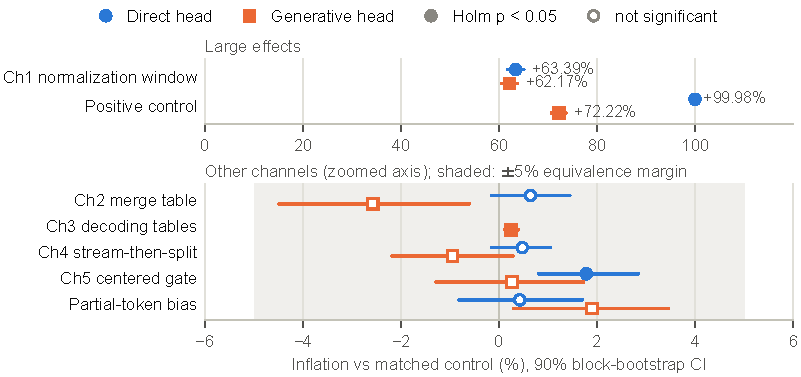
\includegraphics[width=\linewidth]{figures/fig_inflation_folds.pdf}
  \caption{How much each leak inflates accuracy one hour ahead, pooled over the six test periods
  (26,290 forecasts, three training runs). Lines show 90\% bootstrap intervals; filled markers are
  significant after Holm correction; the shaded band marks $\pm5\%$.}
  \label{fig:folds}
\end{figure}

\paragraph{One hour ahead.}
Ch1 dominates (Figure~\ref{fig:folds}): it lowers QLIKE by 63.39\% on the direct head and 62.17\% on
the generative head. Pooling the six periods gives 62.03\% (95\% interval 58.80 to 65.26), with the
same effect in every period ($I^2=0\%$). The other leaks are small. On the direct head they can inflate
accuracy by at most 1.44\% (Ch2), 1.05\% (Ch4) and 2.84\% (Ch5), and Ch3 by at most 0.39\% on the
generative head. Ch5 ($+1.78\%$, Holm $p=0.034$) and Ch3 ($+0.24\%$, Holm $p=0.038$) are detectable
but tiny, and whether they pass the test depends on which training runs are included. Partial-token
bias is not significant one hour ahead ($+0.42\%$ direct, $+1.89\%$ generative).

\begin{table}[t]
  \caption{Boundary leak versus partial-token bias (one training run). QLIKE of the hour-aligned
  reference, the past-only tokenizer and the tokenize-then-cut tokenizer, with $p$-values in
  brackets.}
  \label{tab:tradeoff}
  \centering
  \small
  % Generated by report/make_tables.py from results/ -- do not edit by hand; re-run the script.
\begin{adjustbox}{max width=\linewidth}
\begin{tabular}{lrrrrr}
\toprule
 & \multicolumn{3}{c}{QLIKE (lower is better)} & Partial-token & Boundary \\
\cmidrule(lr){2-4}
Setting & Reference & Context-only & Stream-then-split & bias (\%) & leakage (\%) \\
\midrule
$H{=}288$, Fold 1, seed 0, direct & 0.3128 & 0.3739 & 0.3137 & $-19.53$ ($<$0.001) & $+16.10$ ($<$0.001) \\
2025 holdout, seed 0, direct & 0.4416 & 0.4452 & 0.4494 & $-0.82$ (0.289) & $-0.95$ (0.202) \\
2025 holdout, seed 0, generative & 0.4603 & 0.5538 & 0.4691 & $-20.32$ ($<$0.001) & $+15.30$ ($<$0.001) \\
\bottomrule
\end{tabular}
\end{adjustbox}

\end{table}

\paragraph{One leak can hide another.}
When the cut-short token is costly, the boundary leak wins almost all of the cost back
(Table~\ref{tab:tradeoff}). One day ahead, tokenizing only the past is 19.53\% worse than the
reference, and tokenizing past and future together recovers 16.10\%, ending at 0.3137 against the
reference's 0.3128. The 2025 generative head shows the same pattern. So a leaky pipeline can look as
good as a correct one. Both cases come from a single training run, so we treat this as an observed
pattern rather than a proven effect.

\paragraph{One day ahead, and 2025.}
One day ahead (first period, one run, direct head) every leak grows: Ch1 to 96.36\%, Ch4 to 16.10\%,
Ch5 to 7.02\% and Ch2 to 5.67\% (all Holm $p \le 0.016$). These $p$-values are probably too small:
next-day targets from neighbouring hours overlap by 23 of 24 hours, while our test only allows for
about 7 hours of dependence. On the 2025 test, Ch1 still inflates accuracy by 73.90\% (direct) and
68.32\% (generative). Ch2 changes sign between the two heads ($-5.26\%$ and $+4.93\%$), and Ch5 is not
significant.

\paragraph{Models without leaks.}
On the six periods, the two leak-free GPT direct forecasters are the best models (QLIKE 0.5556 and
0.5580). GARCH (0.5747) is excluded from the confidence set ($p=0.042$), but only when all three
training runs are used; with one run it stays in ($p=0.127$). On 2025 only GARCH remains (0.4267): our
reference GPT (0.4416) beats HAR-RV by 22.08\% but is 3.49\% worse than GARCH. So we measure leakage;
we do not claim a better forecaster.

\paragraph{Extra experiments.}
Letting the normalization window see just $k$ future bars already helps: $+2.70\%$ for one bar (Holm
$p=0.040$), $+6.95\%$ for three and $+18.38\%$ for six (one run). Training on Ethereum data from the
test period adds only $+0.95\%$ (Holm $p=0.188$), while extra Ethereum data from before the test
period adds $+3.06\%$, partly because the model also gets twice as many training steps. Repairing the
cut-short token (token healing) improves the same model's generative forecast by $+1.70\%$ (Holm
$p=0.295$).

% ------------------------------------------------------------------ 5. Discussion and limitations
\section{Discussion and limitations}

Check normalization first: a window that touches the forecast period gives a large, steady and
easy-to-miss boost at both horizons and on 2025, and it is the only leak that beats the best possible
score. The other leaks are small one hour ahead but grow one day ahead, and a tokenize-then-cut
pipeline can hide the cost of a cut-short token. Our study has limits. It covers one asset, with
data from 2021 rather than 2019 as proposed, and a small model trained for five epochs. The next-day,
2025, dose and healing results rest on one training run, and the next-day $p$-values are optimistic.
The partial-token comparison also drops the gate and most volatility tokens, and we did not test
removing the gate or the volatility tokens, as planned at the midterm. All tables and figures are in
our repository.

% ------------------------------------------------------------------ Acknowledgements
\begin{ack}
Prepared for the DA4022 course project (instructor: Prof.\ Ayon Borthakur). Code, results and logs:
\url{https://github.com/devanshjangid2005/causal-vol-tokenizer}.
\end{ack}

% ------------------------------------------------------------------ References
{\small
\bibliographystyle{plainnat}
\bibliography{refs}
}

\end{document}
